\documentclass[tikz,border=2pt]{standalone}
\usepackage{amsmath}
\usetikzlibrary{arrows.meta}
\begin{document}
% A = [[1,2],[2,1]] = P diag(3,-1) P^{-1}, P = [[1,1],[1,-1]]: instead of summing the series for e^{At},
% change to eigenvector coordinates (P^{-1}), multiply by diag(e^{3t}, e^{-t}), and change back (P).
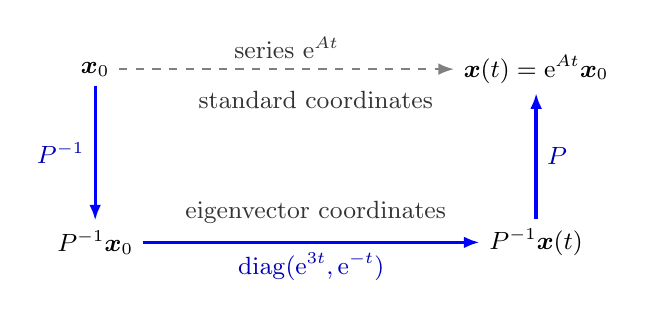
\begin{tikzpicture}[font=\small, >={Latex[length=2mm]}]
  \node (X0) at (0,2.2) {$\boldsymbol{x}_0$};
  \node (Xt) at (5.6,2.2) {$\boldsymbol{x}(t)=\mathrm{e}^{At}\boldsymbol{x}_0$};
  \node (C0) at (0,0) {$P^{-1}\boldsymbol{x}_0$};
  \node (Ct) at (5.6,0) {$P^{-1}\boldsymbol{x}(t)$};
  % direct route: the series
  \draw[->, gray, thick, dashed] (X0) -- (Xt.west)
    node[midway, above, gray!40!black] {series $\mathrm{e}^{At}$};
  % route through the eigenvector coordinates
  \draw[->, blue, very thick] (X0) -- (C0) node[midway, left, blue!70!black] {$P^{-1}$};
  \draw[->, blue, very thick] (C0) -- (Ct)
    node[midway, below, blue!70!black] {$\operatorname{diag}(\mathrm{e}^{3t},\mathrm{e}^{-t})$};
  \draw[->, blue, very thick] (Ct) -- (Xt) node[midway, right, blue!70!black] {$P$};
  % row labels
  \node[gray!40!black, anchor=south] at (2.8,0.12) {eigenvector coordinates};
  \node[gray!40!black, anchor=north] at (2.8,2.05) {standard coordinates};
\end{tikzpicture}
\end{document}
